         \chapter{Analytical geometry}
%     \setcounter{figure}{1}
%     \setcounter{subfigure}{1}
%     \label{71522cd1c95e0cbedb9f300409036b1b}
%          \section{ Cartesian plane \& Distance between two points}
%     \nopagebreak
%             \label{m39107} $ \hspace{-5pt}\begin{array}{cccccccccccc}   
\includegraphics[width=0.75cm]{col11306.imgs/summary_video.png} &   \end{array} $ \hspace{2 pt}\raisebox{-5 pt}{} {(section shortcode: MG10107 )} \par 
%     
%     
%     
%     
%   
%       \label{m39107*uid36}
%             \subsection{ Introduction}
%             \nopagebreak
%             
        \label{m39107*id66769}Analytical geometry, also called co-ordinate geometry and earlier referred to as Cartesian geometry, is the study of geometry using the principles of algebra, and the Cartesian co-ordinate system. It is concerned with defining geometrical shapes in a numerical way, and extracting numerical information from that representation. Some consider that the introduction of analytic geometry was the beginning of modern mathematics.\par 
      \label{m39107*eip-448}
            \section{Drawing figures on the Cartesian plane}
            \nopagebreak
            \label{m39107*eip-728}If we are given the co-ordinates of the vertices of a figure then we can draw that figure on the Cartesian plane. For example take quadrilateral $ABCD$ with co-ordinates: $A(1,1)$, $B(1,3)$, $C(3,3)$ and $D(1,3)$ and represent it on the Cartesian plane. This is shown in Figure~\ref{fig:cartesianplane}.   
\par \label{m39107*eip-199}
    \setcounter{subfigure}{0}
	\begin{figure}[H] % horizontal\label{m39107*id63458}
    \begin{center}
\scalebox{.8}{
\begin{pspicture}(-5,-5)(5.5,5.5)
% \psaxes{<->}(0,0)(5,5)
\psgrid[gridcolor=lightgray,linecolor=lightgray,subgriddiv=1](0,0)(0,0)(4,4)
\psaxes[linewidth=2pt,labels=none,ticks=none]{->}(0,0)(0,0)(5,5)
\pspolygon[linewidth=.1cm](1,1)(1,3)(3,3)(3,1)(1,1)
\uput[dl](1,1){\Large{$A$}}
\uput[dr](3,1){\Large{$B$}}
\uput[ur](3,3){\Large{$C$}}
\uput[ul](1,3){\Large{$D$}}
\uput[l](5.7,0){\Large{$x$}}
\uput[d](0,5.7){\Large{$y$}}
\end{pspicture}
}
\caption{Drawing a figure on the Cartesian plane}
    \end{center}
\label{fig:cartesianplane}
 \end{figure}       
\par \label{m39107*eip-645}To represent any figure on the Cartesian plane, you place a dot at each given co-ordinate and then connect these points with straight lines. One point to note is in naming a figure. In the above example, we called the quadrilateral $ABCD$. This tells us that we move from point $A$, to point $B$, to point $C$, to point $D$ and then back to point $A$ again. So when you are asked to draw a figure on the Cartesian plane, you will follow this naming scheme. If you had the same points, and called it, for example, $ACBD$ you would not get a quadrilateral but a pair of triangles instead. This is important. Sometimes you may be given only some of the points and you will then be required to find the other points using the work covered in the rest of this chapter. \par \label{m39107*uid37}
            \section{ Distance between Two Points}
            \nopagebreak
            \label{m39107*id66786}One of the simplest things that can be done with analytical geometry is to calculate the distance between two points. \Definition{Distance}{Distance is a number that describes how far apart two points are.} For example, point $P$ has co-ordinates $(2,1)$ and point $Q$ has co-ordinates $(-2,-2)$. How far apart are points $P$ and $Q$? In figure~\ref{fig:trianglePQR}, this means how long is the dashed line?\par 
    \setcounter{subfigure}{0}
 	\begin{figure}[H] % horizontal\label{m39107*id63458}
    \begin{center}
\scalebox{.8}{
\begin{pspicture}(-5,-5)(5.5,5.5)
% \psaxes{<->}(0,0)(5,5)
\psgrid[gridcolor=lightgray,linecolor=lightgray,subgriddiv=1](0,0)(-3,-3)(3,3)
\psaxes[linewidth=2pt,labels=none,ticks=none]{->}(0,0)(-3,-3)(3,3)
\psline[linewidth=.1cm](-2,-2)(2,-2)(2,1)
\psline[linestyle=dashed,linewidth=.1cm](-2,-2)(2,1)
\uput[l](-2,-1.8){\Large{$Q$}}
\uput[dl](-1.5,-2){\normalsize{$(-2,-2)$}}
\uput[dr](2,-2){\Large{$R$}}
\uput[u](2.3,0.5){\Large{$P$}}
\uput[ur](2,1){\normalsize{$(2,1)$}}
\uput[l](4,0){\Large{$x$}}
\uput[d](0,4){\Large{$y$}}
\end{pspicture}
}
\caption{Triangle $PQR$}
    \end{center}
\label{fig:trianglePQR}
 \end{figure}        
        \label{m39107*id66883}In figure~\ref{fig:trianglePQR}, it can be seen that the length of the line $PR$ is 3 units and the length of the line $QR$ is four units. However, $\Delta PQR$, has a right angle at $R$. Therefore, the length of the side $PQ$ can be obtained by using the Theorem of Pythagoras:\par 
        \label{m39107*id66950}\nopagebreak\noindent{}          
    \begin{eqnarray*}
     P{Q}^{2} & = & P{R}^{2}+Q{R}^{2} \\ \
\therefore P{Q}^{2} & = & {3}^{2}+{4}^{2} \\ 
\therefore PQ & = & \sqrt{{3}^{2}+{4}^{2}}=5  
      \end{eqnarray*}
        \label{m39107*id67090}The length of $PQ$ is the distance between the points $P$ and $Q$.\par 
        \label{m39107*id67126}In order to generalise the idea, assume $A$ is any point with co-ordinates $({x}_{1};{y}_{1})$ and $B$ is any other point with co-ordinates $({x}_{2};{y}_{2})$.\par 
    \setcounter{subfigure}{0}
 	\begin{figure}[H] % horizontal\label{m39107*id63458}
    \begin{center}
\scalebox{.8}{
\begin{pspicture}(-5,-5)(5.5,5.5)
% \psaxes{<->}(0,0)(5,5)
\psgrid[gridcolor=lightgray,linecolor=lightgray,subgriddiv=1,gridlabels=0.0cm](0,0)(-3,-3)(3,3)
\psaxes[linewidth=1pt,labels=none,ticks=none]{<->}(0,0)(-3,-3)(3,3)
\psline[linewidth=.1cm](-2,-2)(2,-2)(2,1)
\psline[linestyle=dashed,linewidth=.1cm](-2,-2)(2,1)
\uput[l](-2,-1.8){\Large{$A$}}
\uput[dl](-1,-2){\Large{$(x_{1},y_{1})$}}
\uput[dr](2,-2){\Large{$C$}}
\uput[u](2.3,0.5){\Large{$B$}}
\uput[ur](1.8,1){\Large{$(x_{2},y_{2})$}}
\uput[l](4,0){\Large{$x$}}
\uput[d](0,4){\Large{$y$}}
\end{pspicture}
}
    \end{center}
 \end{figure}       
        \label{m39107*id67214}The formula for calculating the distance between two points is derived as follows. The distance between the points $A$ and $B$ is the length of the line $AB$. According to the Theorem of Pythagoras, the length of $AB$ is given by:\par 
        \label{m39107*id67261}\nopagebreak\noindent{}
          
    \begin{equation*}
    AB=\sqrt{A{C}^{2}+B{C}^{2}}
      \end{equation*}
        \label{m39107*id67300}However,\par 
        \label{m39107*id67306}\nopagebreak\noindent{}
          
    \begin{eqnarray*}
     BC & = & {y}_{2}-{y}_{1} \\ AC & = & {x}_{2}-{x}_{1}
      \end{eqnarray*}
        \label{m39107*id67375}Therefore,\par 
        \label{m39107*id67379}\nopagebreak\noindent{}
          
    \begin{eqnarray*} 
AB & = & \sqrt{A{C}^{2}+B{C}^{2}} \\ 
& =& \sqrt{{({x}_{1}-{x}_{2})}^{2}+{({y}_{1}-{y}_{2})}^{2}} 
\end{eqnarray*}
        \label{m39107*id67499}Therefore, for any two points, $\left({x}_{1};{y}_{1}\right)$ and $\left({x}_{2};{y}_{2}\right)$, the formula is:\par 
       \Identity{Distance}{$\mathrm{Distance}=\sqrt{{\left({x}_{1}-{x}_{2}\right)}^{2}+{\left({y}_{1}-{y}_{2}\right)}^{2}}$}
        \label{m39107*id67630}Using the formula, distance between the points $P$ and $Q$ with co-ordinates (2;1) and (-2;-2) is then found as follows. Let the co-ordinates of point $P$ be $\left({x}_{1};{y}_{1}\right)$ and the co-ordinates of point $Q$ be $\left({x}_{2};{y}_{2}\right)$. Then the distance is:\par 
        \label{m39107*id67728}\nopagebreak\noindent{}
          
    \begin{eqnarray*}
\mathsf{Distance} & = & \sqrt{{({x}_{1}-{x}_{2})}^{2} + {({y}_{1}-{y}_{2})}^{2}} \\ 
& =& \sqrt{{(2 - (-2))}^{2} + {(1 - (-2))}^{2}} \\ 
& =& \sqrt{{(2 + 2)}^{2} + {(1+2)}^{2}} \\ 
& =& \sqrt{16 + 9} \\
& =& \sqrt{25} \\ 
& =& 5
      \end{eqnarray*}
        \label{m39107*eip-130}The following video provides a summary of the distance formula.
    \setcounter{subfigure}{0}
	\begin{figure}[H] % horizontal\label{m39107*uid99}
    \textnormal{Khan academy video on distance formula}\vspace{.1in} \nopagebreak
  \label{m39107*yt-media}\label{m39107*yt-video}
            \raisebox{-5 pt}{ 
\includegraphics[width=0.5cm]{col11306.imgs/summary_www.png}} { (Video:  MG10108 )}
      \vspace{2pt}
    \vspace{.1in}
 \end{figure}       \par 
      \label{m39107**end}

\begin{wex}{Distance formula I}{Find the distance between $P(2;1)$ and $Q(-2;-2)$.}{
\westep{Assign values to $(x_1;y_1)$ and $(x_2;y_2)$:}
Let the co-ordinates of $P$ be $(x_1;y_1)$ and the co-ordinates of $Q$ be $(x_2;y_2)$.
\begin{equation*}
 x_1 = 2 \hskip2em y_1 = 1 \hskip2em x_2 = -2 \hskip2em y_2 = -2
\end{equation*}
\westep{Write down the formula you are using:}
\begin{equation*}
 d = \sqrt{(x_1 - x_2)^2 + (y_1 - y_2)^2}
\end{equation*}
\westep{Substitute known variables and solve:}
\begin{equation*}
 \begin{array}{cl}
  d_{\mathrm{PQ}} &= \sqrt{(2 - (-2))^2 + (1 - (-2))^2}\\
  & = \sqrt{(4)^2 + (3)^2}\\
  &= \sqrt{16 + 9}\\
  &= \sqrt{25}\\
  &= 5
 \end{array}
\end{equation*}
\westep{Explain your answer:}
The distance between $P$ and $Q$ is $5$ units.
\vspace{2pt}
    \vspace{.1in}
}
\end{wex}

\begin{wex}{Distance formula II}{Given $RS = 13$, $R(3;9)$ $S(8;y)$, solve for $y$.}{
\westep{Assign values to $(x_1;y_1)$ and $(x_2;y_2)$:}
Let the co-ordinates of $R$ be $(x_1;y_1)$ and the co-ordinates of $S$ be $(x_2;y_2)$.
\begin{equation*}
 x_1 = 3 \hskip2em y_1 = 9 \hskip2em x_2 = 8 \hskip2em y_2 = y
\end{equation*}
\westep{Write down the formula you are using:}
\begin{equation*}
 d = \sqrt{(x_1 - x_2)^2 + (y_1 - y_2)^2}
\end{equation*}
\westep{Substitute known variables and solve:}
\begin{equation*}
 \begin{array}{cl}
  13 &= \sqrt{(3 - 8)^2 + (9 - y)^2}\\
  13^2 & = (-5)^2 + (81 - 18y + y^2)\\
  0 &= y^2 - 18y - 63\\
  &= (y+3) (y-21)\\
 \end{array}
 \therefore y = -3 \hskip1em \mathrm{or} \hskip1em y = 21
\end{equation*}
\westep{Explain your answer:}
$S$ is $(8;-3)$ or $(8;21)$
\vspace{2pt}
    \vspace{.1in}
}
\end{wex}
\begin{exercises}{Distance formula}{
 \begin{enumerate}[label=\textbf{\arabic*}.]
  \item Find the length of $AB$ if:
  \begin{enumerate}
   \item $A(2;7)$ and $B(-3;5)$.
   \item $A(-3;5)$ and $B(-9;1)$.
   \item $A(x;y)$ and $B(x+4;y-1)$.
  \end{enumerate}
  
  \item The length of $CD=5$. Find the missing co-ordinate if:
  \begin{enumerate}
   \item $C(6;-2)$ and $D(x;2)$.
   \item $C(4;y)$ and $D(1;-1)$.
  \end{enumerate}
 \end{enumerate}

 Find the answers with the shortcodes:}
\end{exercises}

%          \section{ Calculation of the gradient line}
%     \nopagebreak
%             \label{m39108} $ \hspace{-5pt}\begin{array}{cccccccccccc}   
\includegraphics[width=0.75cm]{col11306.imgs/summary_video.png} &   \end{array} $ \hspace{2 pt}\raisebox{-5 pt}{} {(section shortcode: MG10109 )} \par 
%     
%     
%     
      \label{m39108*uid40}
            \section{ Gradient of a line}
            \nopagebreak
\label{m39108*id67971}The gradient of a line describes how steep the line is. In the figure, line $PT$ is the steepest. Line $PS$ is less steep than $PT$ but is steeper than $PR$, and line $PR$ is steeper than $PQ$.\par 
    \setcounter{subfigure}{0}
 	\begin{figure}[H] % horizontal\label{m39107*id63458}
    \begin{center}
\scalebox{.8}{
\begin{pspicture}(-5,-5)(5.5,5.5)
% \psaxes{<->}(0,0)(5,5)
\psgrid[gridcolor=lightgray,linecolor=lightgray,subgriddiv=1,gridlabels=0.0cm](0,0)(-1,-1)(4,4)
\psaxes[linewidth=1pt,labels=none,ticks=none]{<->}(0,0)(-1,-1)(4,4)
\psline[linewidth=.05cm](0,0)(1,3.5)
\psline[linewidth=.05cm](0,0)(3,3.5)
\psline[linewidth=.05cm](0,0)(3,2)
\psline[linewidth=.05cm](0,0)(3,0.5)
\uput[ur](.9,3.5){\Large{$T$}}
% \uput[dl](-1,-2){\Large{$(x_{2},y_{2})$}}
\uput[ur](3,3.5){\Large{$S$}}
\uput[ur](3,2){\Large{$R$}}
\uput[ur](3,0.4){\Large{$Q$}}
\uput[dl](0,0){\Large{$P$}}
% \uput[ur](1.8,1){\Large{$(x_{1},y_{1})$}}
\uput[l](4.8,0){\Large{$x$}}
\uput[d](0,4.8){\Large{$y$}}
\end{pspicture}
}
    \end{center}
 \end{figure}        
        \Definition{Gradient}{The gradient of a line is defined as the ratio of the vertical distance to the horizontal distance.} This can be understood by looking at the line as the hypotenuse of a right-angled triangle. Then the gradient is the ratio of the length of the vertical side of the triangle to the horizontal side of the triangle. Consider a line between a point $A$ with co-ordinates $\left({x}_{1};{y}_{1}\right)$ and a point $B$ with co-ordinates $\left({x}_{2};{y}_{2}\right)$.\par 
    \setcounter{subfigure}{0}
 	\begin{figure}[H] % horizontal\label{m39107*id63458}
    \begin{center}
\scalebox{.8}{
\begin{pspicture}(-5,-5)(5.5,5.5)
% \psaxes{<->}(0,0)(5,5)
\psgrid[gridcolor=lightgray,linecolor=lightgray,subgriddiv=1,gridlabels=0.0cm](0,0)(-3,-3)(3,3)
\psaxes[linewidth=1pt,labels=none,ticks=none]{<->}(0,0)(-3,-3)(3,3)
\psline(-2,-2)(2,-2)(2,1)
\psline[linestyle=solid,linewidth=.1cm](-2,-2)(2,1)
\uput[l](-2,-1.8){\Large{$A$}}
\uput[dl](-1,-2){\Large{$(x_{1},y_{1})$}}
\uput[dr](2,-2){\Large{$C$}}
\uput[u](2.3,0.5){\Large{$B$}}
\uput[ur](1.8,1){\Large{$(x_{2},y_{2})$}}
\uput[l](4,0){\Large{$x$}}
\uput[d](0,4){\Large{$y$}}
\end{pspicture}
}
    \end{center}
 \end{figure}  
From this we can obtain the following for the gradient of a line:
\Identity{Gradient}{$\mathsf{gradient} = \frac{y_{2} - y_{1}}{x_{2} - x_{1}}$}
\Tip{We can also use $m$ for the gradient of a line}
\begin{wex}{Gradient I}{Find the gradient of the line between the points E$(2;5)$ and F$(-3;9)$.}{
\westep{Assign values to $(x_1;y_1)$ and $(x_2;y_2)$:}
Let the co-ordinates of E be $(x_1;y_1)$ and the co-ordinates of F be $(x_2;y_2)$.
\begin{equation*}
 x_1 = 2 \hskip2em y_1 = 5 \hskip2em x_2 = -3 \hskip2em y_2 = 9
\end{equation*}
\westep{Write down the formula you are using:}
\begin{equation*}
 m = \frac{y_2 - y_1}{x_2 - x_1}
\end{equation*}
\westep{Substitute known variables and solve:}
\begin{equation*}
 \begin{array}{cl}
  m_{\mathrm{EF}} &= \frac{9 - 5}{-3 - 2}\\
  &= \frac{4}{-5}
 \end{array}
\end{equation*}
\westep{Explain your answer:}
The gradient of $EF = \frac{4}{-5}$
\vspace{2pt}
    \vspace{.1in}
}
\end{wex}


\begin{wex}{Gradient II}{The gradient of $GH = 3$. Find the missing co-ordinate if $G(7;-9)$ and $H(x;0)$.}{
\westep{Assign values to $(x_1;y_1)$ and $(x_2;y_2)$:}
Let the co-ordinates of $G$ be $(x_1;y_1)$ and the co-ordinates of $H$ be $(x_2;y_2)$.
\begin{equation*}
 x_1 = 7 \hskip2em y_1 = -9 \hskip2em x_2 = x \hskip2em y_2 = 0
\end{equation*}
\westep{Write down the formula you are using:}
\begin{equation*}
 m = \frac{y_2 - y_1}{x_2 - x_1}
\end{equation*}
\westep{Substitute known variables and solve:}
\begin{equation*}
 \begin{array}{cl}
  3 &= \frac{0 - (-9)}{x - 7}\\
  3(x-7)&= 9\\
  x-7 &= \frac{9}{3}\\
  x-7 &= 3\\
  x &= 3 + 7\\
  &= 10 \\
 \end{array}
\end{equation*}
\westep{Explain your answer:}
The co-ordinates of $H$ are $(10;0)$.
\vspace{2pt}
    \vspace{.1in}
}
\end{wex}
\begin{exercises}{Gradient Formula}
 \begin{enumerate}
  \item Find the gradient of $AB$ if:
  \begin{enumerate}
   \item $A(7;10)$ and $B(-4;1)$.
   \item $A(-5;-9)$ and $B(3;2)$.
   \item $A(x-3;y)$ and $B(x;y+4)$.
  \end{enumerate}
  
  \item If the gradient of $CD=\frac{2}{3}$, find the missing co-ordinates:
  \begin{enumerate}
   \item $C(16;2)$ and $D(8;y)$.
   \item $C(3;2y)$ and $D(9;14)$.
  \end{enumerate}
 \end{enumerate}

 Find the answers with the shortcodes:
\end{exercises}
  \subsection*{Parallel and Perpendicular Lines}    
%         \label{m39108*eip-332}We can use the gradient of a line to determine if two lines are parallel or perpendicular. If the lines are parallel (Figure~\ref{fig:parallelperpendicular}a) then they will have the same gradient, i.e. ${m}_{\mathrm{AB}}={m}_{\mathrm{CD}}$. If the lines are perpendicular (Figure~\ref{fig:parallelperpendicular}b) than we have: 
%     \setcounter{subfigure}{0}
%  	\begin{figure}[H] % horizontal\label{m39107*id63458}
%     \begin{center}
% \scalebox{.8}{
% \begin{pspicture}(-5,-5)(5.5,5.5)
% % \psaxes{<->}(0,0)(5,5)
% \rput(-2,-2){
% \psline[linewidth=.05cm](0,0)(0,3)
% \psline[linewidth=.05cm](1,0)(1,3)
% \uput[ur](-1,2.8){\Large{$a)$}}
% \uput[d](0,0){\Large{$A$}}
% \uput[u](0,3){\Large{$B$}}
% \uput[d](1,0){\Large{$C$}}
% \uput[u](1,3){\Large{$D$}}}
% 
% \rput(3.4,2){
% \psline[linewidth=.05cm](1,-4)(-2,-1)
% \psline[linewidth=.05cm](-2,-4)(1,-1)
% \uput[ur](-3.2,-1.2){\Large{$b)$}}
% \uput[dr](1,-4){\Large{$A$}}
% \uput[ul](-2,-1){\Large{$B$}}
% \uput[dl](-2,-4){\Large{$C$}}
% \uput[ur](1,-1){\Large{$D$}}}
% \end{pspicture}
% }
%     \end{center}
% \caption{a) Parallel and b) perpendicular lines}
% \label{fig:parallelperpendicular}
%  \end{figure}       
\label{m39108*eip-332}If two lines have equal gradients, it means that the lines are running parallel to each other. In other words: ${gradient}_{\mathrm{AB}}={gradient}_{\mathrm{CD}}$

\begin{wex}{Parallel lines}{Prove that the line $AB$ with points $A(2;4)$ and $B(8,16)$ is parallel to the line $f(x) = 2x-2$.}{
\westep{Find the gradients of both lines:}
\begin{equation*}
 \begin{array}{cl}
  m_{AB} &= \frac{16 - 4}{8 - 2}\\
  &= \frac{12}{6}\\
  &= 2 \\
\\
 m_{f(x)} = 2\\
 \end{array}
\end{equation*}
\westep{Show that they are parallel:}
\begin{equation*}
 m_{AB} = m_{f(x)}
\end{equation*}
\begin{equation*}
 \therefore AB \parallel f(x)
\end{equation*}
}
\end{wex}

Perpendicular lines have gradients that are the negative inverse of each other. This means that when you multiply the gradients together, the answer will be -1. I.e. $-\frac{1}{{m}_{\mathrm{AB}}}={m}_{\mathrm{CD}}$

\begin{wex}{Perpendicular lines}{AB is perpendicular to $CD$. Find $y$ if $A(2;-3)$, $B(-2;6)$, $C(4;3)$ and $D(7;y)$.}{
\westep{Establish how to solve for point $D$:}
\begin{equation*}
 m_{AB} \times m_{CD} = -1
\end{equation*}
\westep{Substitute missing values and solve for point $D$:}
\begin{equation*}
 \begin{array}{rl}
  \frac{6 - (-3)}{-2 -2} \times \frac{y - 3}{7 - 4} &= -1\\
  \frac{9}{-4} \times \frac{y-3}{3} &= -1\\
  \frac{y-3}{3} &= -1 \times \frac{-4}{9}\\
  \frac{y-3}{3} &= \frac{4}{9}\\
  y-3 &= \frac{4}{9} \times 3\\
  y-3 &= \frac{4}{3}\\
  y &= \frac{4}{3} + 3\\
  &= \frac{4 + 9}{3}\\
  &= \frac{13}{3}\\
  &= 4 \frac{1}{3}
 \end{array}
\end{equation*}
\begin{equation*}
 \therefore AB \parallel f(x)
\end{equation*}
}
\end{wex}

\subsection*{Horizontal and Vertical Lines}

When a line runs parallel to the $x$-axis, it is a horizontal line and will have a gradient of zero. This is
because there is no change in the position of the line along the $y$-axis.

When a line runs parallel to the $y$-axis, it is a vertical line. As there is no change in the $x$-values, the
gradient will be undefined.

\subsection*{Collinear Points}

Collinear means to lie on the same line. If a question asks if points are collinear, it is asking if they lie
on the same line. There are two ways to prove this, an easy way using the gradient method, and a
longer method using the distance formula.

If three points are collinear, the line joining them will have the same gradient the whole way across.
This means that if you can prove that any two of the three gradients between the three points are
equal, you can prove that the points are collinear.

\begin{wex}{}{Prove that $A(-3;3)$, $B(0;5)$ and $C(3;7)$ are collinear.}{
\westep{Find any two gradients:}
\begin{equation*}
 m_{AB} = \frac{5-3}{0-(-3)} = \frac{2}{3}
\end{equation*}
\begin{equation*}
 m_{BC} = \frac{7-5}{3-0} = \frac{2}{3}
\end{equation*}
\westep{Establish if the points are collinear and explain your answer:}
\begin{equation*}
 m_{AB} = m_{BC}
\end{equation*}
$\therefore$ Points $A$, $B$ and $C$ are collinear.
}
\end{wex}

To prove that three points are collinear using the distance formula requires finding the
distances between each pair points and then proving that the sum of the two smaller distances
equals the longest distance.

To show this, let's do the same worked example.

\begin{wex}{Collinear points}{Prove that $A(-3;3)$, $B(0;5)$ and $C(3;7)$ are collinear.}{
\westep{Find all three distances:}
\begin{equation*}
 d_{AB} = \sqrt{(-3 - 0)^2 + (3 - 5)^2} = \sqrt{(-3)^2 + (-2)^2} = \sqrt{9 + 4} = \sqrt{13}
\end{equation*}
\begin{equation*}
 d_{BC} = \sqrt{(0 - 3)^2 + (5 - 7)^2} = \sqrt{(-3)^2 + (-2)^2} = \sqrt{9 + 4} = \sqrt{13}
\end{equation*}
\begin{equation*}
 d_{AC} = \sqrt{((-3) - 3)^2 + (3 - 7)^2} = \sqrt{(-6)^2 + (-4)^2} = \sqrt{36 + 16} = \sqrt{52}
\end{equation*}
\westep{Find the sum of the two shorter distances:}
\begin{equation*}
 d_{AB} + d_{BC} = \sqrt{13} + \sqrt{13} = 2\sqrt{13} = \sqrt{4 \times 13} = \sqrt{52}
\end{equation*}
\westep{Prove that the points are collinear:}
\begin{equation*}
 d_{AB} + d_{BC} = d_{AC}
\end{equation*}
$\therefore$ Points $A$, $B$ and $C$ are collinear.
}
\end{wex}

\begin{exercises}{Mixed Gradient Formula}
 \begin{enumerate}
  \item Determine whether $AB$ is parallel, perpendicular or neither to $CD$ if:
  \begin{enumerate}
   \item $A(3;-4)$, $B(5;2)$, $C(-1;-1)$, $D(7;23)$.
   \item $A(3;-4)$, $B(5;2)$, $C(-1;-1)$, $D(0;-4)$.
   \item $A(3;-4)$, $B(5;2)$, $C(-1;-1)$, $D(1;2)$.
  \end{enumerate}
  
  \item Determine whether the following points are collinear:
  \begin{enumerate}
   \item $E(0;3)$, $F(-2;5)$, $G(2;1)$.
   \item $H(-3;-5)$, $I(-0;0)$, $J(6;10)$.
   \item $K(-6;2)$, $L(-3;1)$, $M(1;-1)$.
  \end{enumerate}
 \end{enumerate}
\end{exercises}

        \label{m39108*eip-611}The following video provides a summary of the gradient of a line.
    \setcounter{subfigure}{0}
	\begin{figure}[H] % horizontal\label{m39108*uid993}
    \textnormal{Gradient of a line}\vspace{.1in} \nopagebreak
  \label{m39108*yt-media1}\label{m39108*yt-video1}
            \raisebox{-5 pt}{ 
\includegraphics[width=0.5cm]{col11306.imgs/summary_www.png}} { (Video:  MG10110 )}
      \vspace{2pt}
    \vspace{.1in}
 \end{figure}       \par 
      \label{m39108**end}
%          \section{ Midpoint of a line}
%     \nopagebreak
%             \label{m39119} $ \hspace{-5pt}\begin{array}{cccccccccccc}   
\includegraphics[width=0.75cm]{col11306.imgs/summary_video.png} &   \end{array} $ \hspace{2 pt}\raisebox{-5 pt}{} {(section shortcode: MG10111 )} \par 
%     
%     
%     
      \label{m39119*uid43}
            \section{ Midpoint of a line}
            \nopagebreak
\label{m39119*id68364}Sometimes, knowing the co-ordinates of the middle point or \textsl{midpoint} of a line is useful. For example, what is the midpoint of the line between point $P$ with co-ordinates $(2;1)$ and point $Q$ with co-ordinates $(-2;-2)$.\par 
        \label{m39119*id68433}The co-ordinates of the midpoint of any line between any two points $A$ and $B$ with co-ordinates $({x}_{1};{y}_{1})$ and $({x}_{2};{y}_{2})$, is generally calculated as follows. Let the midpoint of $AB$ be at point $S$ with co-ordinates $(X;Y)$. The aim is to calculate $X$ and $Y$ in terms of $({x}_{1};{y}_{1})$ and $({x}_{2};{y}_{2})$.\par 
    \setcounter{subfigure}{0}
 	\begin{figure}[H] % horizontal\label{m39107*id63458}
    \begin{center}
\scalebox{.8}{
\begin{pspicture}(-5,-5)(5.5,5.5)
\psgrid[gridcolor=lightgray,linecolor=lightgray,subgriddiv=1,gridlabels=0.0cm](0,0)(0,0)(5,5)
\psaxes[linewidth=1pt,labels=none,ticks=none]{->}(0,0)(0,0)(5,5)
\psline[linewidth=.05cm](0,0)(5,5)
\uput[dl](0,0){\Large{$A (x_{1},y_{1})$}}
\uput[u](0,-.2){\qdisk(0,0){3pt}}
\uput[r](2.6,2.4){\Large{$S (X,Y)$}}
\uput[u](2.5,2.3){\qdisk(0,0){3pt}}
\uput[ur](5,5){\Large{$B (x_{2},y_{2})$}}
\uput[u](5,4.8){\qdisk(0,0){3pt}}
\uput[l](5.8,0){\Large{$x$}}
\uput[d](0,5.8){\Large{$y$}}
\end{pspicture}
}
    \end{center}
 \end{figure}      
        \label{m39119*id68637}\nopagebreak\noindent{}
          
    \begin{eqnarray*}
 X & = & \frac{{x}_{1} + {x}_{2}}{2} \\ 
Y & = & \frac{{y}_{1} + {y}_{2}}{2} \\  
      \end{eqnarray*}
From this we obtain the midpoint of a line:
\Identity{Midpoint}{$S(\frac{{x}_{1} + {x}_{2}}{2};\frac{{y}_{1}+{y}_{2}}{2}) $}
        \label{m39119*id68788}Then the co-ordinates of the midpoint ($S$) of the line between point $P$ with co-ordinates $(2;1)$ and point $Q$ with co-ordinates $(-2;-2)$ is:\par 
        \label{m39119*id68860}\nopagebreak\noindent{}
          
    \begin{eqnarray*}
 X & = & \frac{{x}_{1} + {x}_{2}}{2} \\ 
& = & \frac{-2 + 2}{2} \\ 
& = & 0 \\ 
Y & = & \frac{{y}_{1} + {y}_{2}}{2} \\ 
& = & \frac{-2 + 1}{2} \\ 
& = & -\frac{1}{2} 
      \end{eqnarray*}
The midpoint is at $S(0;-\frac{1}{2})$. \\ \pagebreak
        \label{m39119*id69058}It can be confirmed that the distance from each end point to the midpoint is equal. The co-ordinate of the midpoint $S$ is $(0;-0,5)$.\par 
        \label{m39119*id69097}\nopagebreak\noindent{}
          
    \begin{eqnarray*}
PS & = & \sqrt{{({x}_{1} - {x}_{2})}^{2} + {({y}_{1} - {y}_{2})}^{2}} \\ 
& = & \sqrt{{(0 - 2)}^{2} + {(-0,5 - 1)}^{2}} \\ 
& = & \sqrt{{(-2)}^{2} + {(-1,5)}^{2}} \\ 
& = & \sqrt{4 + 2,25} \\ 
& = & \sqrt{6,25}
      \end{eqnarray*}
        \label{m39119*id69323}and\par 
        \label{m39119*id69326}\nopagebreak\noindent{}
          
    \begin{eqnarray*}
QS & = & \sqrt{{({x}_{1} - {x}_{2})}^{2} + {({y}_{1} - {y}_{2})}^{2}} \\ 
& = & \sqrt{{(0 - (-2))}^{2} + {(-0,5 - (-2))}^{2}} \\ 
& = & \sqrt{{(0 + 2)}^{2}{+(-0,5 + 2)}^{2}} \\ 
& = & \sqrt{{(2)}^{2}{+(-1,5)}^{2}} \\ 
& = & \sqrt{4 + 2,25} \\ 
& = & \sqrt{6,25}
      \end{eqnarray*}
        \label{m39119*id69633}It can be seen that $PS=QS$ as expected.\par 
    \setcounter{subfigure}{0}
 	\begin{figure}[H] % horizontal\label{m39107*id63458}
    \begin{center}
\scalebox{.8}{
\begin{pspicture}(-5,-5)(5.5,5.5)
% \psaxes{<->}(0,0)(5,5)
\psgrid[gridcolor=lightgray,linecolor=lightgray,subgriddiv=1,gridlabels=0.0cm](0,0)(-3,-3)(3,3)
\psaxes[linewidth=1pt,labels=none,ticks=none]{->}(0,0)(-3,-3)(3,3)
\psline[linewidth=.05cm](-2,-2)(2,1)
% \psline[linewidth=.05cm](0,0)(3,3.5)
% \psline[linewidth=.05cm](0,0)(3,2)
% \psline[linewidth=.05cm](0,0)(3,0.5)
% \uput[ur](.9,3.5){\Large{$T$}}
\uput[dl](-1,-2){\Large{$Q (-2,-2)$}}
\uput[u](-2,-2.2){\qdisk(0,0){3pt}}
\uput[r](0,-.7){\Large{$S$}}
\uput[r](0,-1.2){\Large{midpoint}}
\uput[u](0,-.7){\qdisk(0,0){3pt}}
\uput[ur](2,1){\Large{$P (2,1)$}}
\uput[u](2,.8){\qdisk(0,0){3pt}}
% \uput[l](4.8,0){\Large{$x$}}
% \uput[d](0,4.8){\Large{$y$}}
\end{pspicture}
}
    \end{center}
 \end{figure} 
       \label{m39119*eip-891}The following video provides a summary of the midpoint of a line.
    \setcounter{subfigure}{0}
	\begin{figure}[H] % horizontal\label{m39119*uid666}
    \textnormal{Khan academy video on midpoint of a line}\vspace{.1in} \nopagebreak
  \label{m39119*yt-media2}\label{m39119*yt-video2}
            \raisebox{-5 pt}{ 
\includegraphics[width=0.5cm]{col11306.imgs/summary_www.png}} { (Video:  MG10112 )}
      \vspace{2pt}
    \vspace{.1in}
 \end{figure}       \par \label{m39119**end}
%          \section{ Summary \& Exercises}
%     \nopagebreak
%             \label{m39167} $ \hspace{-5pt}\begin{array}{cccccccccccc}   \end{array} $ \hspace{2 pt}\raisebox{-0.2em}{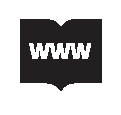
\includegraphics[height=1em]{../icons/www.eps}} {(section shortcode: MG10113 )} \par 
%     
%     
% 
\begin{wex}{Midpoint formula I}{Find the midpoint of line $AB$ if $A$ is at $(6;2)$ and $B$ is at $(-5;-1)$.}{
\westep{Assign values to $(x_1;y_1)$ and $(x_2;y_2)$:}
\begin{equation*}
 x_1= 6 \hskip2em y_1=2 \hskip2em x_2=-5 \hskip y_2=-1
\end{equation*}
\westep{Write down the formula you are using:}
\begin{equation*}
 (\frac{x_1+x_2}{2};\frac{y_1+y_2}{2})
\end{equation*}
\westep{Substitute known variables and solve:}
 \begin{equation*}
  (\frac{6-5}{2};\frac{2-1}{2}) = (\frac{1}{2};\frac{1}{2})
 \end{equation*}
\westep{Explain your answer:}
 $(\frac{1}{2};\frac{1}{2})$ is the midpoint of $AB$.
}
\end{wex}

\begin{wex}{Midpoint formula II}{The line joining $C(-2;4)$ and $D(x;y)$ has the midpoint $M(1;-3)$. Find point $D$.}{
\westep{Assign values to $(x_1;y_1)$ and $(x_2;y_2)$:}
Let the co-ordinates of $C$ be $(x_1;y_1)$ and the co-orindates of $D$ be $(x_2;y_2)$.
\begin{equation*}
 x_1=-2 \hskip2em y_1=4 \hskip2em x_2=x \hskip2em y_2=y
\end{equation*}
\westep{Write down the formula you are using:}
\begin{equation*}
 (\frac{x_1+x_2}{2}; \frac{y_1+y_2}{2})
\end{equation*}
\westep{Substitue known variables and solve:}
\begin{equation*}
 \begin{array}{rllrl}
  1&=\frac{-2+x}{2}&\hskip10em&-3&=\frac{4+y}{2}\\
  1\times 2&=-2+x&&-3\times 2&=4+y\\
  2&=-2+x&&-6&=4+y\\
  x&=2+2&&y&=-6-4\\
  x&=4&&y&=-10\\
 \end{array}
\end{equation*}
\westep{Explain your answer:}
 Point $D$ is at $(4;-10)$.
}
\end{wex}

\begin{wex}{Midpoint formula III}{Points $E(-1;0)$ , $F(0;3)$ , $G(8;11)$ and $H(x;y)$ are points on the Cartesian plane. Find $H(x;y)$ if $EFGH$ is a parallelogram.}{
Remember, the diagonals of a parallelogram bisect each other. This mean that the midpoint of $EG$
will be equal to the midpoint of $FH$. If we find the first midpoint, we can use it to find point $H$.
\westep{For line $EG$, assign values to $(x_1;y_1)$ and $(x_2;y_2)$:}
Let the co-ordinates of $E$ be $(x_1;y_1)$ and the co-orindates of $G$ be $(x_2;y_2)$.
\begin{equation*}
 x_1=-1 \hskip2em y_1=0 \hskip2em x_2=8 \hskip2em y_2=11
\end{equation*}
\westep{Write down the formula you are using:}
\begin{equation*}
 (\frac{x_1+x_2}{2}; \frac{y_1+y_2}{2})
\end{equation*}
\westep{Substitue known variables and solve:}
\begin{equation*}
  (\frac{-1+8}{2}; \frac{0+11}{2}) = (\frac{7}{2};\frac{11}{2})
\end{equation*}
\westep{For line $FH$, assign new values to $(x_1;y_1)$ and $(x_2;y_2)$:}
Let the co-ordinates of $F$ be $(x_1;y_1)$ and the co-orindates of $H$ be $(x_2;y_2)$.
 \begin{equation*}
  x_1=0 \hskip2em y_1=3 \hskip2em x_2=x \hskip2em y_2=y
 \end{equation*}
\westep{Use the midpoint to find H:}
\begin{equation*}
 \begin{array}{rllrl}
  \frac{7}{2}&=\frac{0+x}{2}&\hskip10em&\frac{11}{2}&=\frac{3+y}{2}\\
  7&=x+0&&11&=3+y\\
  x&=7&&y&=8\\
 \end{array}
\end{equation*}
\westep{Explain your answer:}
Point $H$ is at $(7;8)$.
}
\end{wex}

\begin{exercises}{Midpoint Formula}
 \begin{enumerate}
  \item Find the midpoints of the following lines:
  \begin{enumerate}
   \item $A(2;5)$, $B(-4;7)$.
   \item $C(5;9)$, $D(23;55)$.
   \item $E(x+2;y-1)$, $F(x-5;y-4)$.
  \end{enumerate}
  
  \item The midpoint $M$ of $PQ$ is (3;9). Find $P$ is $Q$ is $(-2;5)$:

  \item $MNOP$ is a parallelogram with the points $M(5;3)$, $N(2;1)$ and $O(7;-3)$. Find point $P$.
 \end{enumerate}
\end{exercises}    
  \label{m39167*fs-id5760712}
            \section{ Summary }
            \nopagebreak
\label{m39167*fs-id1165371842904}
\label{m39167*eip-966}\begin{itemize}[noitemsep]
            \item Figures can be represented on the Cartesian plane\item The formula for finding the distance between two points is: \label{m39167*eid9734}\nopagebreak\noindent{}
    \begin{equation}
    \mathsf{Distance}=\sqrt{{\left({x}_{1}-{x}_{2}\right)}^{2}+{\left({y}_{1}-{y}_{2}\right)}^{2}}
      \end{equation}
    \item The formula for finding the gradient of a line is: \label{m39167*edi6342}\nopagebreak\noindent{}
    \begin{equation}
    \mathsf{Gradient}=\frac{{y}_{2}-{y}_{1}}{{x}_{2}-{x}_{1}}
      \end{equation}
    \item The formula for finding the midpoint between two points is: \label{m39167*eid6743}\nopagebreak\noindent{}
    \begin{equation}
    S\left(\frac{{x}_{1}+{x}_{2}}{2};\frac{{y}_{1}+{y}_{2}}{2}\right)
      \end{equation}
\item  If two lines are parallel then they will have the same gradient, i.e. ${m}_{\mathsf{AB}}={m}_{\mathsf{CD}}$. If two lines are perpendicular than we have: $-\frac{1}{{m}_{\mathsf{AB}}}={m}_{\mathsf{CD}}$\end{itemize}
\par 
\label{m39167*secfhsst!!!underscore!!!id2370}
            \section{ End of Chapter exercises}
            \nopagebreak
        \label{m39167*id69671}\begin{enumerate}[noitemsep, label=\textbf{\arabic*}. ] 
            \label{m39167*uid43466}\item 
Represent the following figures on the Cartesian plane: \label{m39167*id6549695}\begin{enumerate}[noitemsep, label=\textbf{\alph*}. ] 
            \label{m39167*uid4746}\item Triangle $DEF$ with $D(1;2)$, $E(3;2)$ and $F(2;4)$ 
\label{m39167*uid4548}\item Quadrilateral $GHIJ$ with $G(2;-1)$, $H(0;2)$, $I(-2;-2)$ and $J(1;-3)$
\label{m39167*uid4549}\item Quadrilateral $MNOP$ with $M(1;1)$, $N(-1;3)$, $O(-2;3)$ and $P(-4;1)$ 
\label{m39167*uid5450}\item Quadrilateral $WXYZ$ with $W(1;-2)$, $X(-1;-3)$, $Y(2;-4)$ and $Z(3;-2)$
\end{enumerate}
                \label{m39167*uid46}\item 
In the diagram given the vertices of a quadrilateral are $F(2;0)$, $G(1;5)$, $H(3;7)$ and $I(7;2)$.
    \setcounter{subfigure}{0}
 	\begin{figure}[H] % horizontal\label{m39107*id63458}
    \begin{center}
\scalebox{.8}{
\begin{pspicture}(-5,-5)(5.5,5.5)
% \psaxes{<->}(0,0)(5,5)
\psgrid[gridcolor=lightgray,linecolor=lightgray,subgriddiv=1](0,0)(-1,-1)(7,7)
\psaxes[linewidth=1pt,labels=none,ticks=none]{->}(0,0)(-1,-1)(7,7)
\pspolygon[linewidth=.05cm,fillstyle=solid,fillcolor=lightgray](2,0)(1,5)(3,7)(7,2)(2,0)
% \psline[linewidth=.05cm](0,0)(3,3.5)
% \psline[linewidth=.05cm](0,0)(3,2)
% \psline[linewidth=.05cm](0,0)(3,0.5)
% \uput[ur](.9,3.5){\Large{$T$}}
\uput[d](2,-.2){\normalsize{$F (2,0)$}}
\uput[ul](1.2,5){\normalsize{$G (1,5)$}}
\uput[u](3,7){\normalsize{$H (3,7)$}}
\uput[r](7,2){\normalsize{$I (7,2)$}}
\uput[l](8,0){\Large{$x$}}
\uput[d](0,8){\Large{$y$}}
\end{pspicture}
}
    \end{center}
 \end{figure}  
       \label{m39167*id69695}\begin{enumerate}[noitemsep, label=\textbf{\alph*}. ] 
            \label{m39167*uid47}\item 
What are the lengths of the opposite sides of $FGHI$?
\label{m39167*uid48}\item Are the opposite sides of $FGHI$ parallel?
\label{m39167*uid49}\item  Do the diagonals of $FGHI$ bisect each other?
\label{m39167*uid50}\item  Can you state what type of quadrilateral $FGHI$ is? Give reasons for your answer.
\end{enumerate}
                \label{m39167*uid51}\item 
A quadrialteral $ABCD$ with vertices $A(3;2)$, $B(1;7)$, $C(4;5)$ and $D(1;3)$ is given.
\label{m39167*id69770}\begin{enumerate}[noitemsep, label=\textbf{\alph*}. ] 
            \label{m39167*uid52}\item  Draw the quadrilateral.
\label{m39167*uid53}\item  Find the lengths of the sides of the quadrilateral.
\end{enumerate}
                \label{m39167*uid54}\item $ABCD$ is a quadrilateral with verticies $A(0;3)$, $B(4;3)$, $C(5;-1)$ and $D(-1;-1)$.
\label{m39167*id69816}\begin{enumerate}[noitemsep, label=\textbf{\alph*}. ] 
            \label{m39167*uid55}\item Show that:
\label{m39167*id69834}\begin{enumerate}[noitemsep, label=\textbf{\roman*}. ] 
            \label{m39167*uid56}\item $AD = BC$
\label{m39167*uid57}\item $AB \parallel DC$
\end{enumerate}
        \label{m39167*uid58}\item What name would you give to $ABCD$?
\label{m39167*uid59}\item Show that the diagonals $AC$ and $BD$ do not bisect each other.
\end{enumerate}
                \label{m39167*uid60}\item $P$, $Q$, $R$ and $S$ are the points $(-2;0)$, $(2;3)$, $(5;3)$, $(-3;-3)$ respectively.
\label{m39167*id69919}\begin{enumerate}[noitemsep, label=\textbf{\alph*}. ] 
            \label{m39167*uid61}\item Show that:
\label{m39167*id69937}\begin{enumerate}[noitemsep, label=\textbf{\roman*}. ] 
            \label{m39167*uid62}\item $SR = 2PQ$
\label{m39167*uid63}\item $SR \parallel PQ$
\end{enumerate}
        \label{m39167*uid64}\item Calculate:
\label{m39167*id69993}\begin{enumerate}[noitemsep, label=\textbf{\roman*}. ] 
            \label{m39167*uid65}\item $PS$
\label{m39167*uid66}\item $QR$
\end{enumerate}
        \label{m39167*uid67}\item What kind of a quadrilateral is $PQRS$? Give reasons for your answers.
\end{enumerate}
                \label{m39167*uid68}\item $EFGH$ is a parallelogram with verticies $E(-1;2)$, $F(-2;-1)$ and $G(2;0)$. Find the co-ordinates of H by using the fact that the diagonals of a parallelogram bisect each other.\newline
\item  
$PQRS$ is a quadrilateral with points $P(0;-3)$ ; $Q(-2;5)$ ; $R(3;2)$ and $S(3;-2)$  in the Cartesian plane.
\label{m39167*id0812312}\begin{enumerate}[noitemsep, label=\textbf{\alph*}. ] 
            \label{m39167*id08123}\item Find the length of $QR$.
\label{m39167*id981221}\item Find the gradient of $PS$.
\label{m39167*id08213}\item Find the midpoint of $PR$.
\label{m39167*id9871293}\item Is $PQRS$ a parallelogram?  Give reasons for your answer. \end{enumerate}
                \item $A(-2;3)$ and $B(2;6)$ are points in the Cartesian plane. $C(a;b)$ is the midpoint of $AB$. Find the values of $a$ and $b$.
\item 
Consider: Triangle $ABC$ with vertices $A(1; 3)$ , $B(4;1)$ and $C (6; 4)$:
\label{m39167*id9173123}\begin{enumerate}[noitemsep, label=\textbf{\alph*}. ] 
            \item Sketch triangle $ABC$ on the Cartesian plane. 
\item Show that $ABC$ is an isoceles triangle.
\item Determine the co-ordinates of $M$, the midpoint of $AC$.
\item Determine the gradient of $AB$.
\item Show that the following points are collinear: $A$, $B$ and $D(7;-1)$
\end{enumerate}
\item In the diagram, $A$ is the point $(-6;1)$ and $B$ is the point $(0;3)$
    \setcounter{subfigure}{0}
 	\begin{figure}[H] % horizontal\label{m39107*id63458}
    \begin{center}
\scalebox{.8}{
\begin{pspicture}(-5,-5)(5.5,5.5)
% \psaxes{<->}(0,0)(5,5)
\psgrid[gridcolor=lightgray,linecolor=lightgray,subgriddiv=1](0,0)(-10,-1)(1,7)
\psaxes[linewidth=1pt,labels=none,ticks=none]{->}(0,0)(-10,-1)(1,7)
\psline[linewidth=.05cm](-6,1)(0,3)
% \psline[linewidth=.05cm](0,0)(3,3.5)
% \psline[linewidth=.05cm](0,0)(3,2)
% \psline[linewidth=.05cm](0,0)(3,0.5)
% \uput[ur](.9,3.5){\Large{$T$}}
\uput[d](-6,1){\Large{$A (-6,1)$}}
\uput[d](-5.9,1.2){\qdisk(0,0){3pt}}
\uput[ul](-.2,3){\Large{$B (0,3)$}}
\uput[d](0,3.2){\qdisk(0,0){3pt}}
\uput[l](1.8,0){\Large{$x$}}
\uput[d](0,8){\Large{$y$}}
\end{pspicture}
}
    \end{center}
 \end{figure} 
      \label{m39167*id982373}\begin{enumerate}[noitemsep, label=\textbf{\alph*}. ] 
            \item Find the equation of line $AB$ 
\item Calculate the length of $AB$
\item  $A'$ is the image of $A$ and $B'$ is the image of $B$. Both these images are obtain by applying the transformation: $(x;y)\to(x - 4;y - 1)$. Give the coordinates of both $A'$ and $B'$
\item Find the equation of $A'B'$
\item Calculate the length of $A'B'$
\item Can you state with certainty that $AA'B'B$ is a parallelogram? Justify your answer.\end{enumerate}
                 \end{enumerate}
\label{m39167**end}
  \label{71522cd1c95e0cbedb9f300409036b1b**end}
\par \raisebox{-0.2em}{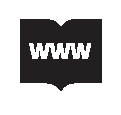
\includegraphics[height=1em]{../icons/www.eps}} Find the answers with the shortcodes:
 \par \begin{tabular}[h]{cccccc}
 (1.) lgv  &  (2.) liZ  &  (3.) liB  &  (4.) lac  &  (5.) lax  &  (6.) laa  &  (7.) laY  &  (8.) lag  &  (9.) la4  &  (10.) l4o  & \end{tabular}
